\documentclass{beamer}
\usetheme{Berkeley}
\title{RSA Cryptography: Our World's Security}
\author{Seth Hamilton}
\usecolortheme{default}
\usepackage{tikz}
\usepackage{graphicx}
\DeclareGraphicsExtensions{.jpg}
\institute{Valparaiso University}
\begin{document}
\begin{frame}
\titlepage
\end{frame}
\begin{frame}
\tableofcontents
\end{frame}
\section{Motivation}
\begin{frame}
\frametitle{Motivation}
\begin{itemize}
\item During my freshman year, I heard a talk on Cryptography.
\item The presentation was very interesting and blended the ideas of computer science with mathematics.
\item The Imitation Game was also a part in my interest in encryption and decryption of codes.
\end{itemize}
\end{frame}
\section{History}
\begin{frame}
\frametitle{History}
\begin{itemize}
\item Cryptography is the subject of transforming information, so it cannot be easily recovered without special knowledge. 
\item Julius Caesar is one of the first known people to use cryptography.
\item He shifted the letters of the alphabet in order to encrypt messages he was sending. 
\item Originally, cryptography would be a system that could be represented as a receiver receiving many messages (locks) and having to keep track of many different keys that go to these locks in order to break them. 
\end{itemize}
\end{frame}
\begin{frame}
\frametitle{History}
\begin{itemize}
\item James Ellis came up with an idea that would allow a public distribution of open locks all with the same key, but the locks could have a message kept inside then sent back to the person with the key so only he/she can open the lock and read the message.
\item Sadly, Ellis was unable to come up with a mathematical solution to his idea.
\end{itemize}
\end{frame}
\begin{frame}
\frametitle{History}
\begin{itemize}
\item Ronald Rivest, Adi Shamir, and Leonard Adleman perfected public key cryptography or what we call RSA.
\end{itemize}
\begin{center}
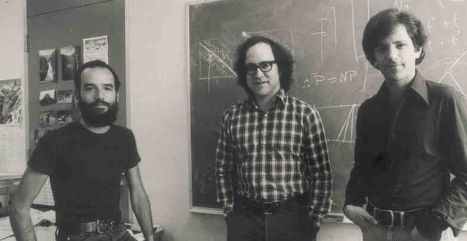
\includegraphics[width=4in, height=2in]{RSA.jpg}\\
\end{center}
\end{frame}
\section{How RSA Works}
\begin{frame}
\frametitle{Receiver}
\begin{itemize}
\item 1. First, the receiver picks 2 very large primes, $p$ and $q$. Also, compute $n=pq$.
\item 2. Compute $m=lcm (p-1, q-1)$. 
\item 3. Pick an $e$ relatively prime to $m$. 
\item 4, Find $d$ such that $ed \mod m=1$.
\item 5. Announce $n$ and $e$ publicly. \\
NOTE: Each $p$ and $q$ are 100-200 digits each and $n$ is anywhere between 200 and 400 digits.
\end{itemize}
\end{frame}
\begin{frame}
\frametitle{Example}
\begin{itemize}
\item As the receiver, choose two primes, say 37 and 73. Compute the product, which is 2701.
\item Compute the lcm of 36 and 72, which is 72. 
\item Choose an $e$ relatively prime to 72, say 7. 
\item Find a $d$ such that $7d \mod 72=1$. Thus, $d=31$.
\end{itemize}
\end{frame}

\begin{frame}
\frametitle{Sender}
\begin{itemize}
\item 1. Convert the message to a string of digits.
\item 2. Break up the message into uniform blocks of digits; call them $M_1, M_2, ... , M_k$.
\item 3. Calculate and send $R_i=M_i^e \mod n$.
\end{itemize}
\end{frame}
\begin{frame}
\frametitle{Example}
Suppose I want to send the message "YES"
\begin{itemize}

\item As the sender, convert the letters into a string of digits. Use a code for each of the 26 letters starting with a=01 through z=26 and blank with 00.
\item We have 250519.
\item Now, break these up into strings of length 4. This gives strings $M_1= 2505, M_2=1900$.
\item Compute $R_1=2505^7 \mod 2701=692$, $R_2=1900^7 \mod 2701=1734$.
\item The sender will send 0692 and 1734.
\end{itemize}
\end{frame}

\begin{frame}
\frametitle{Receiver}
\begin{itemize}
\item 1. For each received message, $R_i$, calculate $R_i^d \mod n$.
\item 2. Convert the string of digits back to a string of characters.
\end{itemize}
\end{frame}
\begin{frame}
\frametitle{Example}
\begin{itemize}
\item 0692 and 1734 will be received.
\item As the receiver, now compute $692^{31} \mod 2701=2505$ and $1734^{31} \mod 2701=1900$.
\item Now convert 25051900 back to letters to decrypt the message.
\item We know each letter is encoded with a two-digit number.
\item Split 25051900 into blocks of 2.
\item This gives 25 (Y), 05 (E), 19 (S). 
\end{itemize}
\end{frame}
\begin{frame}
\frametitle{Mod Simplification}
\begin{itemize}
\item Consider $692^{31}$. If we were to compute this, we get a number 89 digits long.
\item Take $692^{31}=(692^2)^{8} (692^3)^5$. The numbers are much smaller and easier to deal with. 
\item $692^{31} \mod 2701 \equiv ((692^2 \mod 2701)^8 \mod 2701)\cdot$ $((692^3 \mod 2701)^5 \mod 2701) \mod 2701 $
\item We only have $692^2$ and $692^3$, which are 6 and 9 digits, instead of 89. 
\item Now, to mod out by 2701, the problem is quicker by far.
\end{itemize}
\end{frame}
\section{Proof}
\begin{frame}
\frametitle{Proof}
\begin{block}{Fermat's Little Theorem}
If $p$ is any prime number, and $a$ is any integer such that $p \nmid a$, then $a^{p-1}\equiv 1\mod p$. \\
\end{block}
\begin{block}{Chinese Remainder Theorem}
A system of linear congruences modulo pairwise relatively prime integers has a unique solution modulo the product of these moduli.\\
\end{block}
\end{frame}
\begin{frame}
\frametitle{Proof}
\begin{itemize}
\item Assume $de \equiv 1\mod (p-1)(q-1)$. Then, there exists an integer, $k$, such that $de=1+k(p-1)(q-1)$. 
\item It follows that\\
 $R^d\equiv (M^e)^d=M^{de}=M^{1+k(p-1)(q-1)}\mod n$.
\item $gcd(M, p)=gcd(M,q)=1 \Rightarrow M^{p-1}\equiv 1 \mod p$ and $M^{q-1} \equiv 1 \mod q$. 
\item Therefore, $R^d \equiv M \cdot (M^{p-1})^{k(q-1)}\equiv M\cdot 1 = M \mod p$
\item Also, $R^d \equiv M \cdot (M^{q-1})^{k(p-1)}\equiv M\cdot 1 = M \mod q$
\item $gcd(p, q)=1 \Rightarrow R^d\equiv M\mod pq$.
\end{itemize}
\end{frame}
\section{Future Work}
\begin{frame}
\frametitle{Future Work}
\begin{itemize}
\item RSA can fuel more research around prime numbers.
\item That being said, if someone figures out a way to factor large numbers into two primes rather quickly, security will be compromised.
\item Some non-secret forms of communication, such as email, can be used between the sender and receiver to speed up the process since the RSA process is time consuming.
\item Until 2007, RSA gave cash prizes for factoring large numbers into two primes. 
\end{itemize}
\end{frame}
\section{References}
\begin{frame}
\frametitle{References}
\begin{thebibliography}{99}

\bibitem{Ro} K. H. Rosen, \underline{Discrete Mathematics and Its Applications 7th Edition}, Monmouth University, 2007.
\bibitem{Ep} S. Epp, \underline{Discrete Mathematics with Applications 4th Edition}, Brooks/Cole, 2011.
\bibitem{Ha} Public Key Cryptography: RSA Encryption Algorithm, \\ \url{https://www.youtube.com/watch?v=wXB-V_Keiu8}
Princeton University Press, 2008.

\end{thebibliography}

\end{frame}
\begin{frame}
\begin{center}
\begin{itemize}
\item Thanks to Professor Beagley for advising me on this project!
\item Thanks to you all for being here!
\item For any further questions or comments, email me at seth.hamilton@valpo.edu.
\end{itemize}
\end{center}
\end{frame}
\end{document}
